\documentclass{../c-lecture}

\usepackage{algorithm2e}

\subtitle{Repeating Statements}

\begin{document}

\begin{frame}
  \titlepage{}
\end{frame}
\begin{frame}
  \frametitle{Outline}
  \tableofcontents{}
\end{frame}

\section{Introduction}

\begin{frame}
  \frametitle{Repetition}
  \begin{itemize}
    \item Example: Write a program that read 3 integer and compute average
    \begin{itemize}
      \item It is easy. 3 scanf, an addition, a division and, a printf
    \end{itemize}
    \item Example: Write a program that read 3000 integer and compute average
    \begin{itemize}
      \item 3000 scanf!!!?
    \end{itemize}
    \item Example: Write a program that read n integer and compute average
    \begin{itemize}
      \item N??? scanf
    \end{itemize}
  \end{itemize}
\end{frame}

\begin{frame}
  \frametitle{Repetition: counter controlled}
  \begin{itemize}
    \item When we know the number of iteration
    \begin{itemize}
      \item Average of 10 number
    \end{itemize}
  \end{itemize}
  \begin{algorithm}[H]
  \KwData{}
  \KwResult{}
  $counter \gets 0$\;

  \While{$counter < number\_of\_loop\_repetition$}{%
    do something (e.g.\ read input, take sum)\;
    $counter \gets counter + 1$\;
  }
  \end{algorithm}
\end{frame}

\begin{frame}
  \frametitle{Repetition: sentinel controlled}
  \begin{itemize}
    \item
      When we do \textbf{\color{RubineRed} NOT} know the number of iteration
    \item But we know, when loop terminates
    \begin{itemize}
      \item E.g. Average of arbitrary positive numbers ending with < 0
    \end{itemize}
  \end{itemize}
  \begin{algorithm}[H]
  \KwData{}
  \KwResult{}
  $n \gets$ get first input\;

  \While{$n != sentinel$}{%
    do something (sum, \ldots)\;
    $n \gets$ get the next input\;
    \eIf{there is not any valid input}{%
      S1
    }{%
      S2
    }
  }
  \end{algorithm}
\end{frame}

\begin{frame}
  \frametitle{Repetition}
  \begin{itemize}
    \item Repetition is performed by loops
    \begin{itemize}
      \item
        Put all statements to repeat in a \textbf{\color{Orange} loop}
    \end{itemize}
    \item Don’t loop to infinity
    \begin{itemize}
      \item Stop the repetition
      \item Based on some conditions (counter, sentinel)
    \end{itemize}
    \item C has three statements for loops
    \begin{itemize}
      \item \textit{\color{Orange} while} statement
      \item \textit{\color{Orange} do-while} statement
      \item \textit{\color{Orange} for} statement
    \end{itemize}
  \end{itemize}
\end{frame}

\section{while statement}

\begin{frame}[fragile]
  \frametitle{while statement}
  \begin{minted}[bgcolor=Black]{c}
while ( <expression> )
  <statements>
  \end{minted}
\end{frame}

\begin{frame}[fragile]
  \frametitle{print 0 to n}
  \begin{minted}[bgcolor=Black]{c}
#include <stdio.h>

int main(void) {
  int n, number;
  number = 0;
  printf("Enter n: ");
  scanf("%d", &n);
  while(number <= n) {
    printf("%d \n", number);
    number++;
  }
  return 0;
}
  \end{minted}
\end{frame}

\section{do-while statement}

\begin{frame}[fragile]
  \frametitle{do-while statement}
  \begin{minted}[bgcolor=Black]{c}
do {
  <statements>
} while ( <expression> );
  \end{minted}
\end{frame}

\begin{frame}[fragile]
  \frametitle{sum of the n term: 1/2 + 2/3 \ldots}
  \scriptsize
  \begin{minted}[bgcolor=Black]{c}
#include <stdio.h>

int main(void) {
  int n;
  double number, sum;

  printf("Enter n > 0: ");
  scanf("%d", &n);

  if(n < 1){
    printf("wrong input");
    return -1;
  }

  sum = 0;
  number = 0.0;
  do {
    number++;
    sum += number / (number + 1.0);
  } while(number < n);

  printf("sum = %lf\n", sum);
  return 0;
}
  \end{minted}
\end{frame}

\begin{frame}[fragile]
  \frametitle{sum of the inputs until zeor}
  \scriptsize
  \inputminted[bgcolor=Black]{c}{./src/do-while-read.c}
\end{frame}

\section{for statement}

\begin{frame}[fragile]
  \frametitle{for statement}
  \begin{minted}[bgcolor=Black]{c}
for(<expression1>; <expression2>; <expression3>)
  <statements>
  \end{minted}
\end{frame}

\begin{frame}
  \frametitle{for statement}
  \begin{enumerate}
    \item The delaration, definition, and initialization of the \textbf{loop variable(s)}
    \item A \textbf{loop condition} which specifies how long the for iteration should continue.
    \begin{itemize}
      \item The loop condition is checked before each execution of the loop body.
    \end{itemize}
    \item Another statement which is executed after each iteration.
  \end{enumerate}
\end{frame}

\begin{frame}[fragile]
  \frametitle{N students average grade}
  \scriptsize
  \begin{minted}[bgcolor=Black]{c}
#include <stdio.h>

int main(void) {
  int grade, count, i;
  double average, sum;
  sum = 0;
  printf("Enter the number of students: ");
  scanf("%d", &count);
  for(i = 0; i < count; i++) {
    printf("Enter the grade of %d-th student: ", (i + 1));
    scanf("%d", &grade);
    sum += grade;
  }
  average = sum / count;
  printf("The average of your class is %0.3lf\n", average);
  return 0;
}
  \end{minted}
\end{frame}

\begin{frame}[fragile]
  \frametitle{Expressions in for statements}
  \begin{itemize}
    \item
      Expression1 and Expression3 can be any number of expressions, they execute
      in the order
    \begin{minted}[bgcolor=Black]{c}
for(i = 0, j = 0; i < 10; i++, j--)
    \end{minted}
    \item Expression2 at most should be a single expression
    \item
      If multiple expressions then the value of the last one is evaluated as
      True/False
    \begin{minted}[bgcolor=Black]{c}
for(i = 0, j = 0; i < 10, j > -100; i++, j--)
    \end{minted}
  \end{itemize}
\end{frame}

\begin{frame}[fragile]
  \frametitle{Expressions in for statements}
  \begin{itemize}
    \item Any expression can be empty expression
    \begin{minted}[bgcolor=Black]{c}
for( ; i < 10; i++)
for(;;)
    \end{minted}
  \end{itemize}
\end{frame}

\begin{frame}[fragile]
  \frametitle{Loop Variable}
  \begin{itemize}
    \item
      Often, people place the definition of the loop variable somewhere before the for or even
      reuse variable for several loops.
    \item \textbf{\color{RubineRed} DON'T} do that.
    \item to help occasional reader and the compiler understand your code
    \item it is important to know that this variable has the special meaning of an iteration counter for that given for loop
  \end{itemize}
  \begin{minted}[bgcolor=Black]{c}
for(int i = 0; i < 10; i++)
  \end{minted}
\end{frame}

\section{Arrays}

\begin{frame}
  \frametitle{Introduction}
  \begin{itemize}
    \item Algorithms usually work on large data sets
    \begin{itemize}
      \item Sort a set of numbers
      \item Search a specific number in a set of numbers
    \end{itemize}
    \item How to read and store a set of data?
    \item To Read
    \begin{itemize}
      \item Repeat the \textit{scanf} statement
      \item Use the loop statements
    \end{itemize}
    \item To store the data
    \begin{itemize}
      \item Save each data in a single variable??
      \item 3000 int variables!!!!
    \end{itemize}
  \end{itemize}
\end{frame}

\begin{frame}
  \frametitle{Array}
  \begin{itemize}
    \item
      An \textit{\color{Orange} ordered} collection of
      \textit{\color{Orange} same type} variables

    \item A $1 x n$ vector of
    \begin{itemize}
      \item Integers, chars, floats, \ldots
    \end{itemize}
    \item Example
    \begin{itemize}
      \item An array of 8 integers
      \begin{table}
      \begin{tabular}{*{8}{c}}
        \toprule

        0 &
        1 &
        2 &
        3 &
        4 &
        5 &
        6 &
        7 \\

        \midrule

        3 &
        1 &
        5 &
        11 &
        10 &
        19 &
        0 &
        12 \\

        \bottomrule
      \end{tabular}
      \end{table}
      \item An array of 5 chars
      \begin{table}
      \begin{tabular}{*{5}{c}}
        \toprule

        0 &
        1 &
        2 &
        3 &
        4 \\

        \midrule

        a &
        z &
        F &
        z &
        k \\

        \bottomrule
      \end{tabular}
      \end{table}
    \end{itemize}
  \end{itemize}
\end{frame}

\begin{frame}[fragile]
  \frametitle{Arrays in C}
  \begin{itemize}
    \item Array declaration in C
    \begin{minted}[bgcolor=Black]{c}
      <Elements’ Type> <identifier>[<size>]
    \end{minted}
    \begin{minted}[bgcolor=Black]{c}
      int arr[20]
    \end{minted}
    \item
      \mintinline{c}|<Elements’ Type>|: int, char, float,
      \ldots
    \item \mintinline{c}|<size>|
    \begin{itemize}
      \item Old compilers (standard): it should be constant
      \item New compilers (standard): it can be variable
    \end{itemize}
    \item Elements in array
    \begin{itemize}
      \item From 0 to (size – 1)
    \end{itemize}
  \end{itemize}
\end{frame}

\begin{frame}[fragile]
  \frametitle{Example}
  \begin{minted}[bgcolor=Black]{c}
    int num[20]
  \end{minted}
  \begin{itemize}
    \item num is array of 20 integers
    \item num[0] is the first integer variable
    \item num[19] is the last integer
  \end{itemize}
  \begin{minted}[bgcolor=Black]{c}
    float farr[100]
  \end{minted}
  \begin{itemize}
    \item farr is array of 100 floats
    \item farr[0] is the first float
    \item farr[49] is the 50th float
    \item farr[99] is the last float
  \end{itemize}
\end{frame}

\begin{frame}[fragile]
  \frametitle{Array Initialization: Known Length}
  \begin{itemize}
    \item \mint{c}|int num[3]={10, 20, 60};|
    \begin{itemize}
      \item num is the array of 3 integers, \mintinline{c}|num[0]| is 10, \ldots
    \end{itemize}

    \item \mint{c}|int num[]={40, 50, 60, 70, 70, 80};|
    \begin{itemize}
      \item num is the array of 6 integers
    \end{itemize}

    \item \mint{c}|int num[10]={40, 50, 60};|
    \begin{itemize}
      \item num is the array of 10 integers
      \item \mintinline{c}|num[0]| is 40, \mintinline{c}|num[1]| is 50, \mintinline{c}|num[2]| is 60
      \item \mintinline{c}|num[3], num[4], ..., num[9]| are 0
    \end{itemize}
  \end{itemize}
\end{frame}

\begin{frame}[fragile]
  \frametitle{Array Initialization (cont’d)}
  \begin{minted}[bgcolor=Black]{c}
int num[2]={40, 50, 60, 70};
/* Compile warning */

int num[5]={[0] = 3, [4] = 6};
/* num[5] = {3, 0, 0, 0, 6} */
  \end{minted}
\end{frame}

\begin{frame}[fragile]
  \frametitle{Initializing Variable Length Arrays}
  \begin{minted}[bgcolor=Black]{c}
int n;
scanf("%d", &n);
int num[n]={0}; /* Compile error */
  \end{minted}
  \begin{block}{}
    Variable length arrays cannot be initialized!
  \end{block}
  \begin{minted}[bgcolor=Black]{c}
for(i = 0; i < n; i++)
  num[i] = 0;
  \end{minted}
\end{frame}

\begin{frame}[fragile]
  \frametitle{Variable Length Array Declaration}
  \begin{minted}[bgcolor=Black]{c}
int n;
scanf("%d", &n);
int num[n];
  \end{minted}
  \textit{\color{Orange} num} is usable
  \begin{minted}[bgcolor=Black]{c}
int n;
int num[n];
scanf("%d", &n);
  \end{minted}
  \begin{block}{}
    \textit{\color{Orange} num} is
    \textit{\color{RubineRed} not} usable, why?
  \end{block}
\end{frame}

\section{Advanced loops}

\begin{frame}[fragile]
  \frametitle{Empty statements}
  \begin{itemize}
    \item <statement> in loops can be empty
  \end{itemize}
  \begin{minted}[bgcolor=Black]{c}
while(<expression>) ;
E.g.,
while(i++ <= n) ;

for(<expression1>; <expression2>; <expression3>) ;
E.g.,
for(i = 0; i < 10; printf("%d\n",i), i++) ;
  \end{minted}
\end{frame}

\begin{frame}[fragile]
  \frametitle{Nested loops}
  \begin{itemize}
    \item <statement> in loops can be loop itself
  \end{itemize}
  \begin{minted}[bgcolor=Black]{c}
while(<expression0>)
  for(<expression1>; <expression2>; <expression3>)
    <statements>
  \end{minted}
  \begin{minted}[bgcolor=Black]{c}
for(<expression1>; <expression2>; <expression3>)
  do
    <statements>
  while(<expression>)
  \end{minted}
\end{frame}

\begin{frame}[fragile]
  \frametitle{Nested loops example}
  \begin{itemize}
    \item A program that takes n and m and prints
    \begin{minted}[bgcolor=Black]{output}
*** ...* (m * in each line)
*** ...*
...
*** ...*
(n lines)
    \end{minted}
  \end{itemize}
\end{frame}

\begin{frame}[fragile]
  \begin{minted}[bgcolor=Black]{c}
#include <stdio.h>

int main(void){
  int i, j, n, m;
  printf("Enter n & m: ");
  scanf("%d %d", &n, &m);

  for(i = 0; i < n; i++){
    for(j = 0; j < m; j++) {
      printf("*");
    }
    printf("\n");
  }
  return 0;
}
  \end{minted}
\end{frame}

\begin{frame}[fragile]
  \frametitle{Nested loops example}
  \begin{itemize}
    \item A program that takes n and prints
    \begin{minted}[bgcolor=Black]{output}
* (i * in i-th line)
**
***
*** ...*
(n lines)
    \end{minted}
  \end{itemize}
\end{frame}

\begin{frame}[fragile]
  \begin{minted}[bgcolor=Black]{c}
#include <stdio.h>

int main(void) {
  int i, j, n;
  printf("Enter n: ");
  scanf("%d", &n);

  i = 1;
  while(i <= n) {
    for(j = 0; j < i; j++) {
      printf("*");
    }
    printf("\n");
    i++;
  }
  return 0;
}
  \end{minted}
\end{frame}

\begin{frame}[fragile]
  \frametitle{break statement}
  \begin{itemize}
    \item Exit from loop based on some conditions
  \end{itemize}
  \begin{minted}[bgcolor=Black]{c}
do{
  scanf("%d", &a);
  scanf("%d", &b);

  if(b == 0)
    break;

  res = a / b;
  printf("a / b = %d\n", res);
} while(b > 0);
  \end{minted}
\end{frame}

\begin{frame}[fragile]
  \frametitle{continue statement}
  \begin{itemize}
    \item Jump to end of loop and continue repetition
  \end{itemize}
  \begin{minted}[bgcolor=Black]{c}
do {
  scanf("%f", &a);
  scanf("%f", &b);
  if(b == 0)
    continue;
  res = a / b;
  printf("a / b = %f\n", res);
} while(a > 0);
  \end{minted}
\end{frame}

\begin{frame}
  \frametitle{Which loop?}
  \begin{itemize}
    \item When you know the number of repetition
    \begin{itemize}
      \item Counter-controlled loops
      \item Usually, \textit{\color{Orange} for} statements
    \end{itemize}
    \item When you don’t know the number of repetitions (sentinel loop)
    \begin{itemize}
      \item Some condition should be check before starting loop
      \begin{itemize}
        \item Usually, \textit{\color{LimeGreen} while} statement
      \end{itemize}
      \item The loop should be executed at least one time
      \begin{itemize}
        \item Usually, \textit{\color{Cyan} do-while}
      \end{itemize}
    \end{itemize}
  \end{itemize}
\end{frame}

\section{Bugs and avoiding them}

\begin{frame}[fragile]
  \frametitle{Common bugs and avoiding them}
  \begin{itemize}
    \item Loop should terminate
    \begin{itemize}
      \item
        e.g., in for loops, after each iteration, we should approach to the stop
        condition
    \end{itemize}
    \begin{minted}[bgcolor=Black]{c}
for(i = 0; i < 10; i++) // ok
for(i = 0; i < 10; i--) // bug
    \end{minted}
    \item Initialize loop control variables
    \begin{minted}[bgcolor=Black]{c}
int i;
for( ; i < 10; i++)
    \end{minted}
  \end{itemize}
\end{frame}

\begin{frame}[fragile]
  \frametitle{Common bugs and avoiding them}
  \begin{itemize}
    \item \textbf{\color{RubineRed} Don’t modify} for loop controller in loop body
    \begin{minted}[bgcolor=Black]{c}
for(i = 0; i < 10; i++) {
  ...
  i--; // bug
}
    \end{minted}
    \item Take care about wrong control conditions
    \begin{itemize}
      \item{< vs. <=}
      \item{= vs. ==}
    \end{itemize}
    \begin{minted}[bgcolor=Black]{c}
int b = 10;
int a = 0;
while(a = b) { // it means while(true)
  scanf("%d", &a)
}
    \end{minted}
  \end{itemize}
\end{frame}

\begin{frame}
  \frametitle{Legends}
  \begin{figure}
    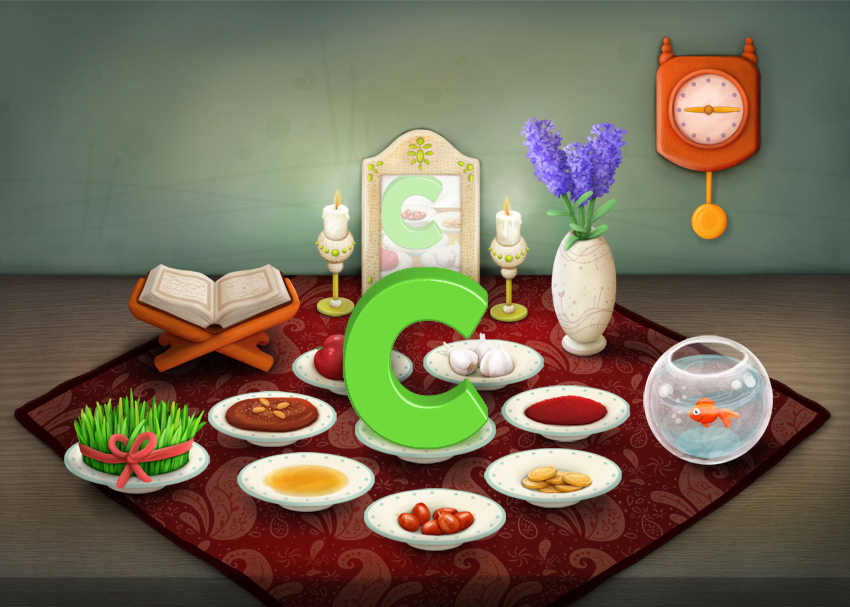
\includegraphics[width=.75\textwidth]{./img/nowruz.jpg}
  \end{figure}
  \pause%
  \centering
  \color{Violet} Happy Nowruz
\end{frame}

\end{document}
